\documentclass{article} 
\usepackage{fullpage, hyperref, amsmath, amssymb, graphicx, graphics, float, listings, color} 
\usepackage[dvipsnames]{xcolor}

\begin{document} 
\title{Team Snails Documentation - DECO 3801\\
Chris Flores, Harry Guthrie, Joshua Hwang, Richard Marron, Michael Delmastro, Leo Orpilla III} 
\maketitle 

\tableofcontents

\newpage

\section{Introduction}
	
	This report will cover the planning and development of a chosen task by Team Sails. 
	
	\subsection{Project Description}
		The chosen project by Team Snails was ``{\it Challenge of Designing Large Interactive Public Displays}" by the Tie Han Han team. As the title suggests, this project will be targeting the challenge of creating large public displays which would be put up in places like the UQ campus for example, from which students or visitors can interact with the display. 

	\subsection{Outline of Goals}
		The goals set out by the team were:
		\begin{itemize}
			\item Create a display application which handles the displaying of relevant information and messages while also looking good on a large screen.
				\begin{itemize}
					\item Lay down a solid foundation for the back-end to support this type of application.
					\item Have a robust database to hold relevant information
					\item Create useful APIs to help development.
				\end{itemize}
			\item Develop a mobile application which can communicate with the display app so that the user may interact with the large display.
				\begin{itemize}
					\item Have a way for the mobile app to talk to the display app through a server.
					\item Make sure there is security for logins and protecting user data.
				\end{itemize}
			\item Improve the overall design and user experience for both applications.
		\end{itemize}

\section{Team Structure}
	
	The first task of the project was to structure the team in such a way to make development easier. This was achieved by splitting the team into two groups; the front-end team and the back-end team. 
	
	\subsection{Front-End Team \& Goals}
		The front-end team was designated to develop user interfaces (UI) which includes graphical design and human computer interaction (HCI). The team consisted of Richard, Leo and Michael who worked on the aforementioned tasks. Richard and Michel began to design the graphical interface by taking HCI theory into consideration and improving on the design provided in the specification, while Leo worked on the implementation of user interaction with the UI. The front-end team decided to focus on delivering a great user experience and satisfying design with dynamic elements. 

	\subsection{Back-End Team \& Goals}
		The back-end is all about creating a robust foundation to support the required functionality and the interface designed by the front-end team. Team members of the back-end team were Chris, Harry and Josh who - like the front-end team - split themselves to work on different aspects of the project to increase efficiency. Harry worked on setting up developer operations and the overall structure of the back-end whilst also running the production server and working on the uqcloud box. Chris and Josh focussed on developing the back-end for Flask and ensuring that the team had a solid application programming interface (API) for the team to utilise.

\section{Features}
	
	\subsection{Implemented Features}
		This section will cover the included features which were successfully implemented, and will also cover features which were discussed during feature  but were ultimately cut from the project due to either too large of a scope or limited time.
	\subsection{Cut Features}
		\begin{itemize}
			\item Booking library study rooms from the application 
			\item Checking book availability
		\end{itemize}
	
		\subsubsection{Reasoning}

\section{Progression}	
	This section details how the project has progressed through development.
	\subsection{Front-End Progression}
		Prototyping phase commenced 10th August 2020 with some rough sketches - see Figure \ref{proto}.
		\begin{figure}[h!]
			\centering
			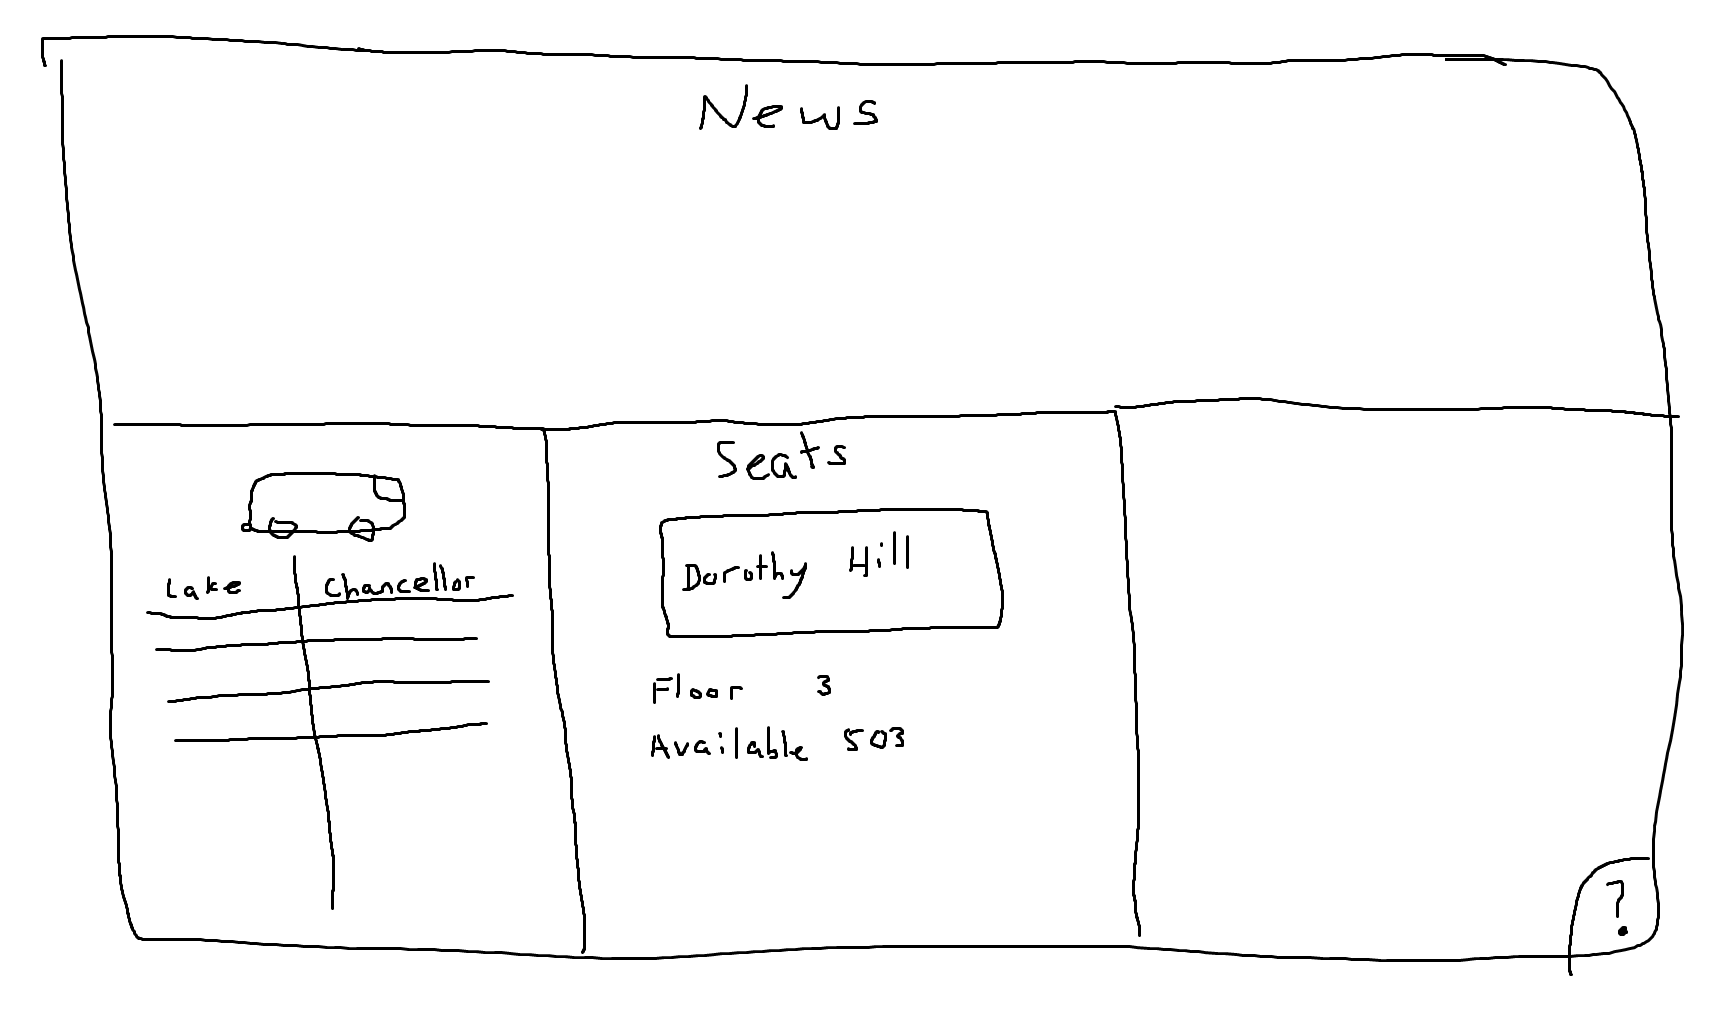
\includegraphics[width=0.8\textwidth]{Figures/prototype.png}
			\caption{Initial rough sketch - 10/08/20}
			\label{proto}
		\end{figure}
		Although, the front-end team decided that this format does not facilitate enough information for what they were trying to achieve, and therefore refined the user interface (UI) to allow this. Figure \ref{proto2} shows this refinement. \\
		\newpage
		\begin{figure}[h!]
			\centering
			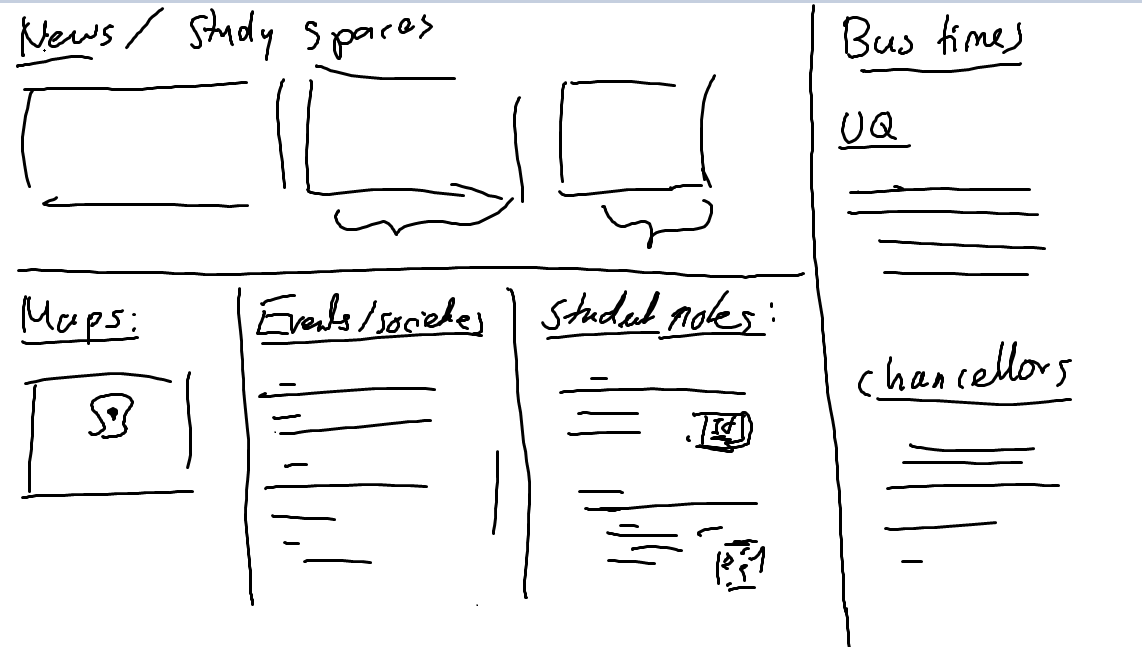
\includegraphics[width=0.8\textwidth]{Figures/prototype2.png}
			\caption{Stage 1 Refinement - 10/08/20}
			\label{proto2}
		\end{figure}
		Working further on this layout, they created a more polished iteration of the front-end which concludes the sketching phase. The front-end team also added in placeholder data which helps visualise what will be shown on the display. \\
		
		\begin{figure}[h!]
			\centering
			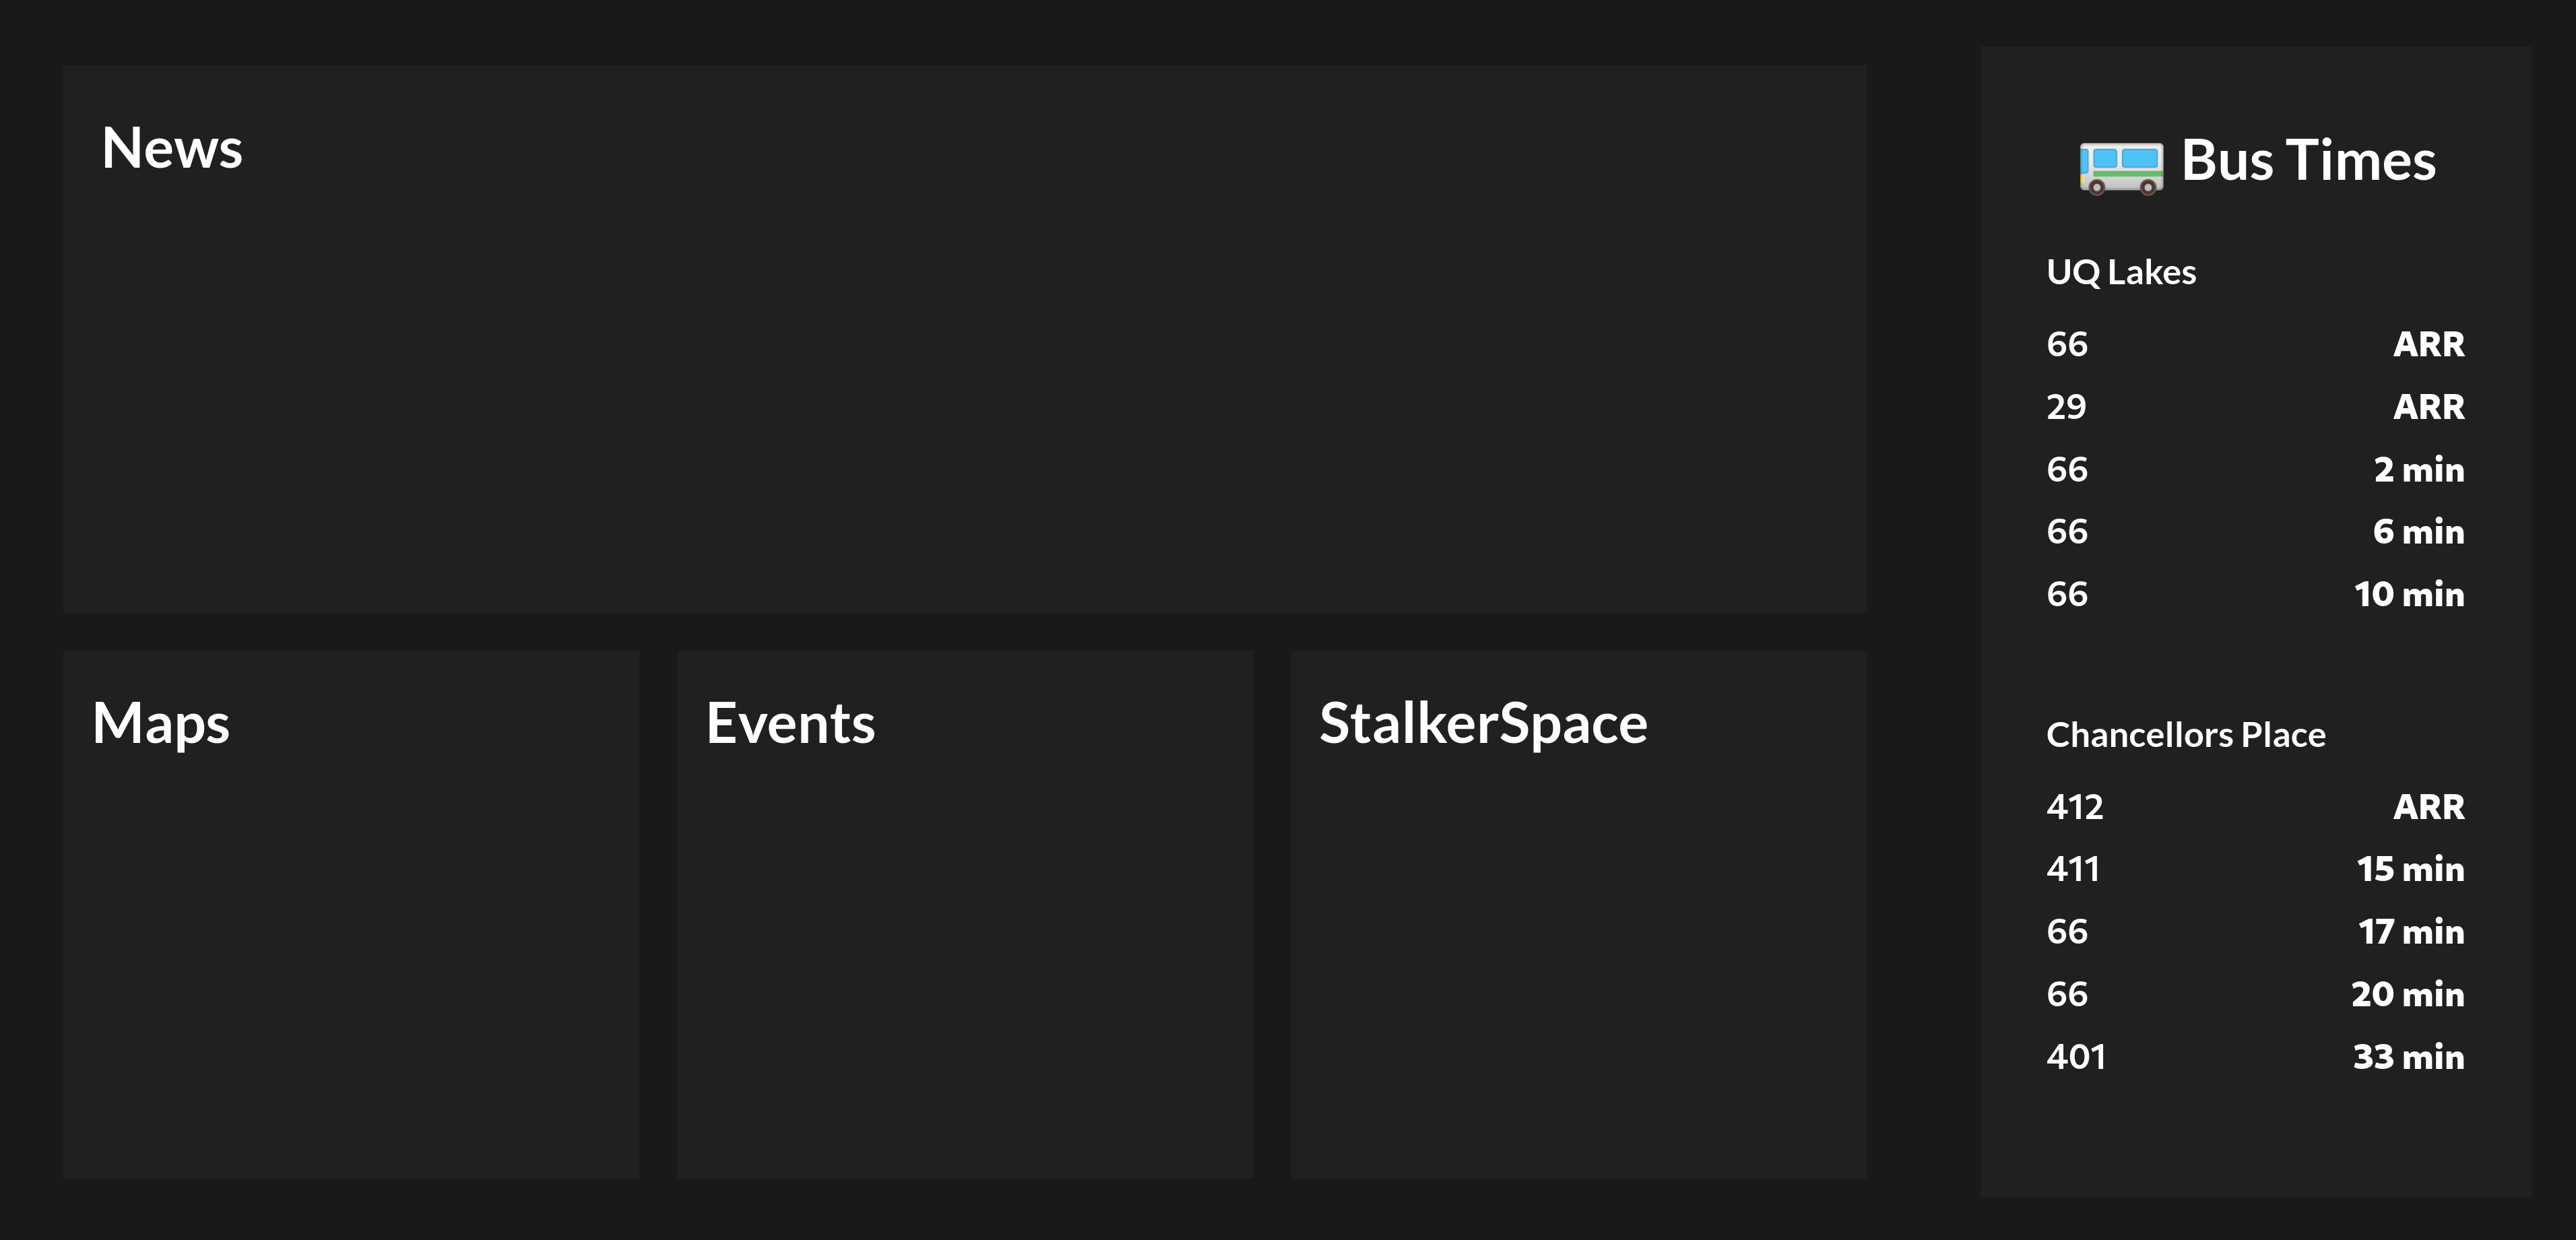
\includegraphics[width=0.8\textwidth]{Figures/prototype3.png}
			\caption{Improving Front-end - 10/08/20}
			\label{proto3}
		\end{figure}
		After constructing the UI in Figure \ref{proto3}, colour was added to flesh out some of the ``panels" for the display which is shown in Figure \ref{proto4}.
		\begin{figure}[H]
			\centering
			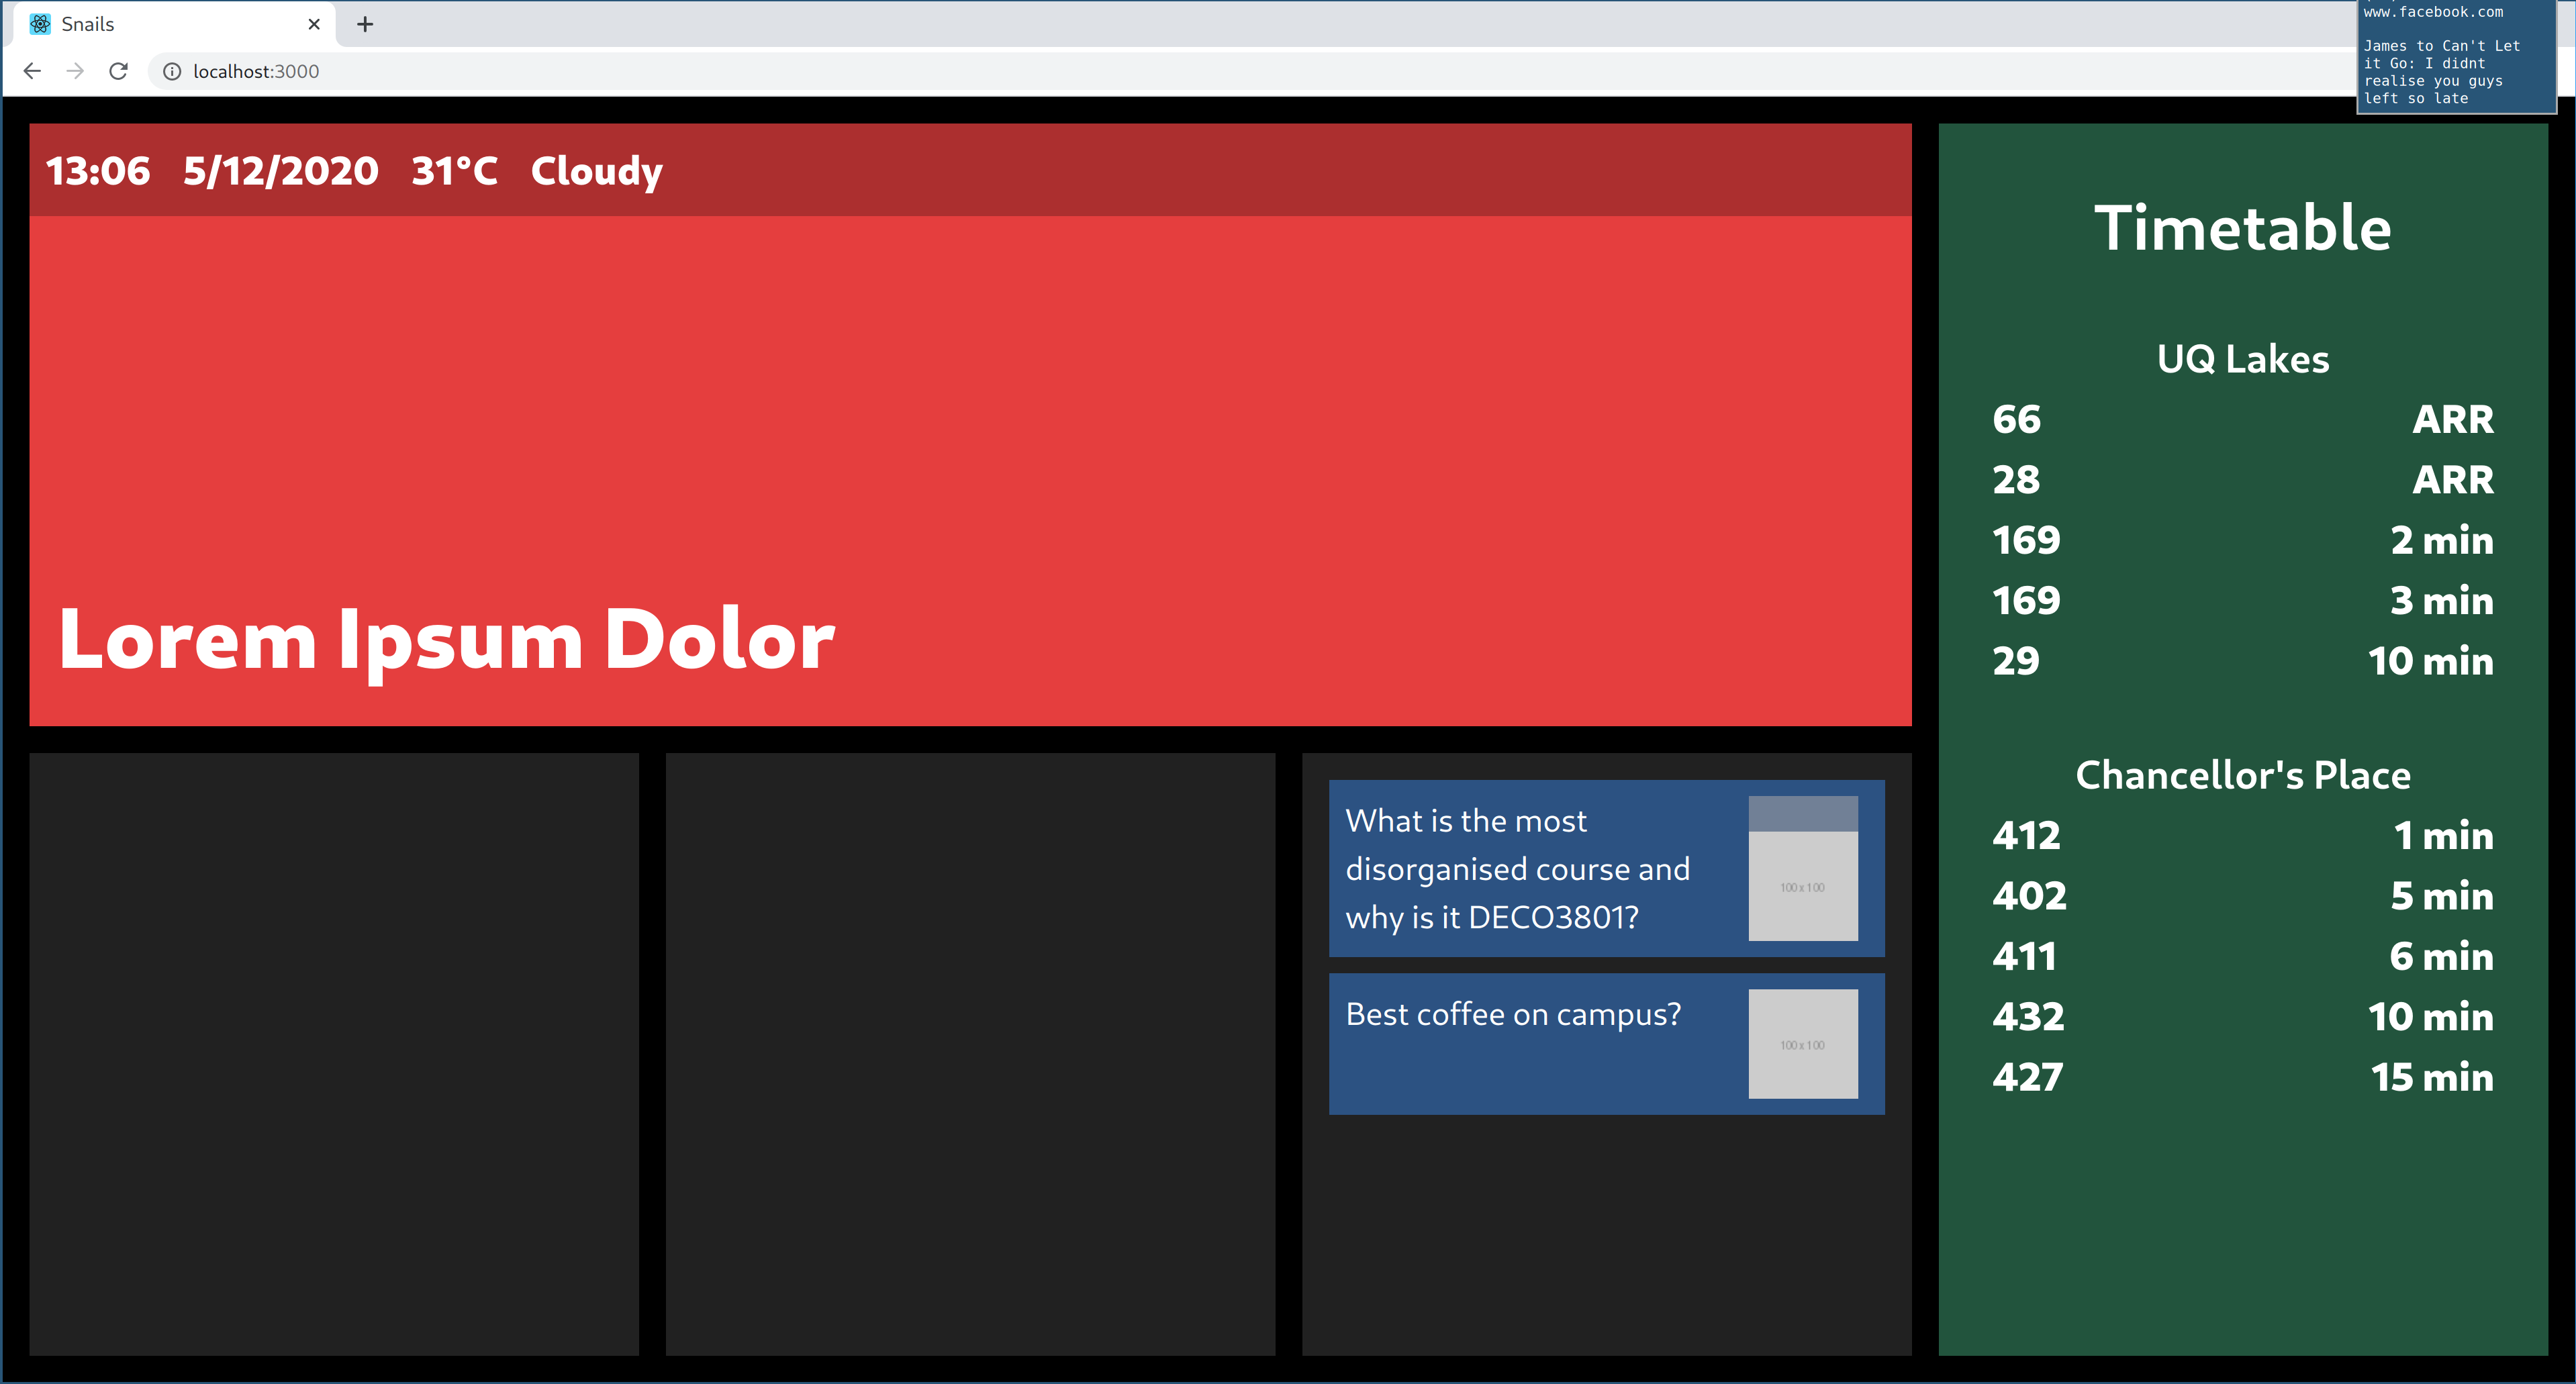
\includegraphics[width=0.8\textwidth]{Figures/prototype4.png}
			\caption{Adding Colour to the Interface - 11/08/20}
			\label{proto4}
		\end{figure}
		As of 12th August 2020, the team experimented with different display aspect ratios and orientations. This is to ensure that no matter what device the program is running on, the interface will still look correct and no information is lost. Figure \ref{proto5} is one such attempt at designing the interface to adapt for displays with square aspect ratios. \\
		
		\begin{figure}[h!]
			\centering
			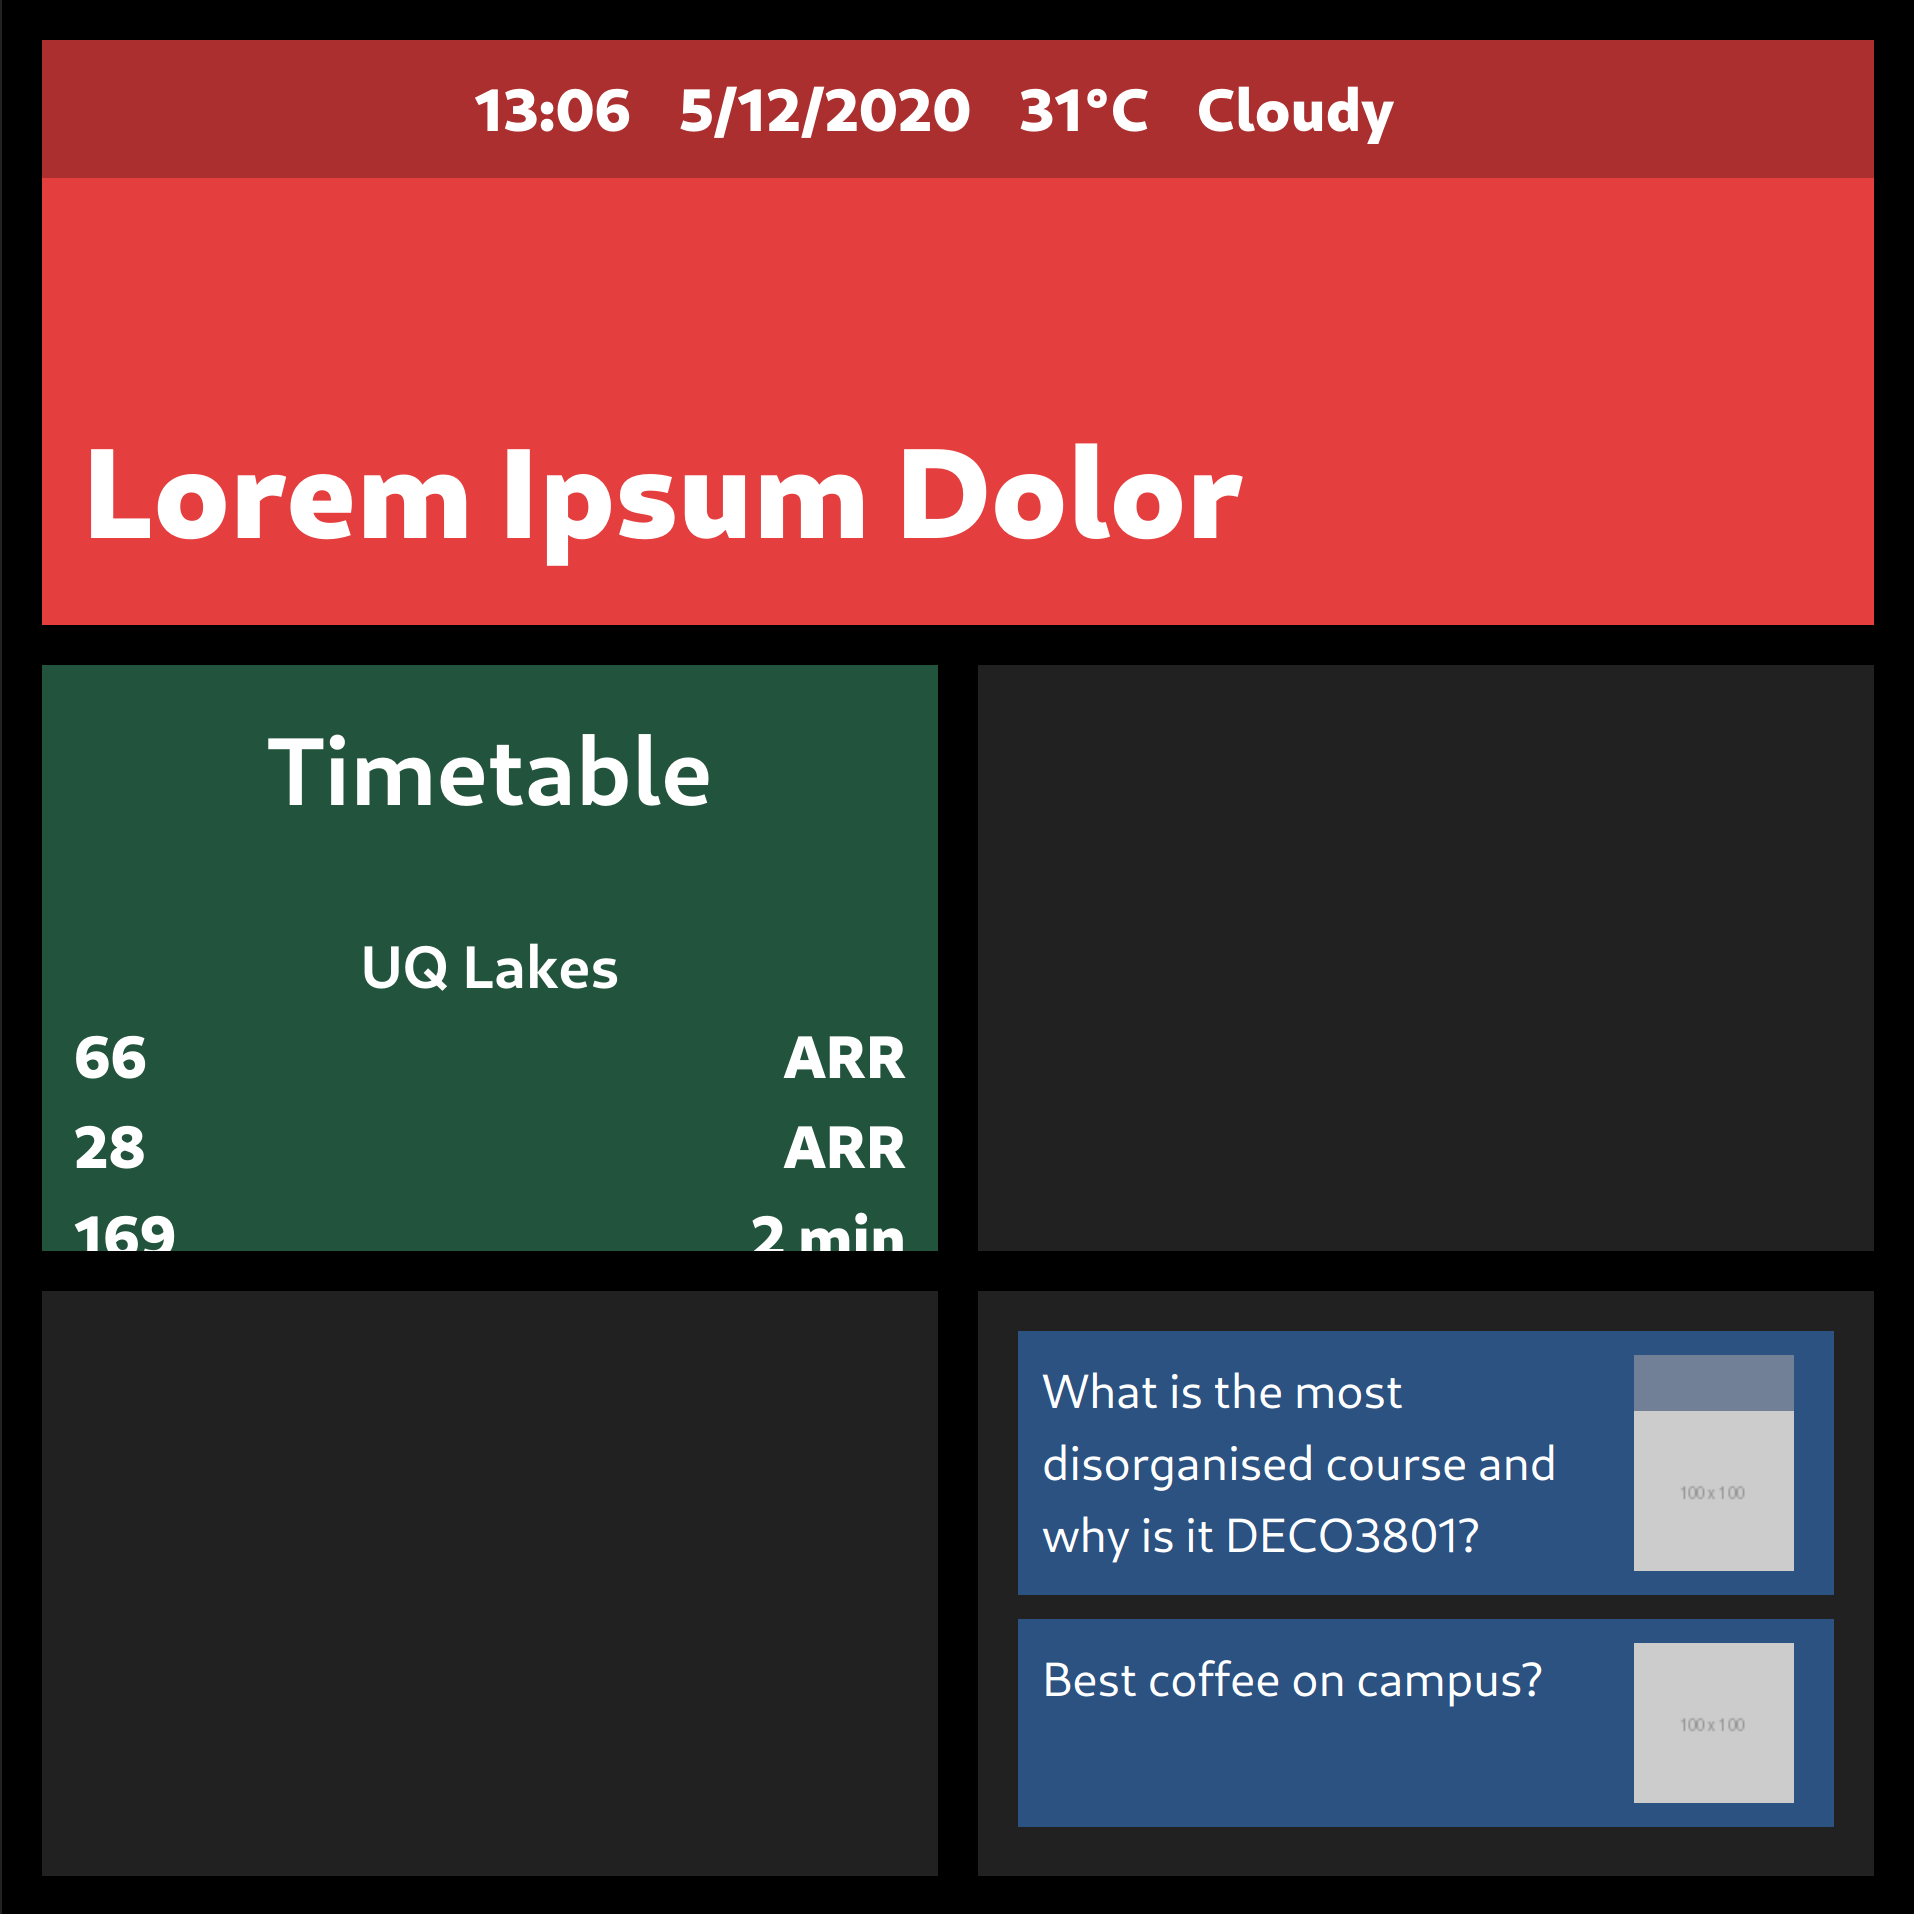
\includegraphics[width=0.5\textwidth]{Figures/prototype5.png}
			\caption{Square Aspect Ratio Display - 12/08/20}
			\label{proto5}
		\end{figure}
		From the figure, the bus timetable panel on the display is truncated and not all of the information is shown. This was altered in subsequent iterations however the team thought about having the text scroll so that it shows the hidden information. The idea was eventually scrapped. \\
		
		From the middle of week 2 onwards, the front-end team focused on colour schemes and resizeable panels on the display. An example was made which ``looks very UQ-like" which can be seen in Figure \ref{UQlike}. \\
		
		\begin{figure}[h!]
			\centering
			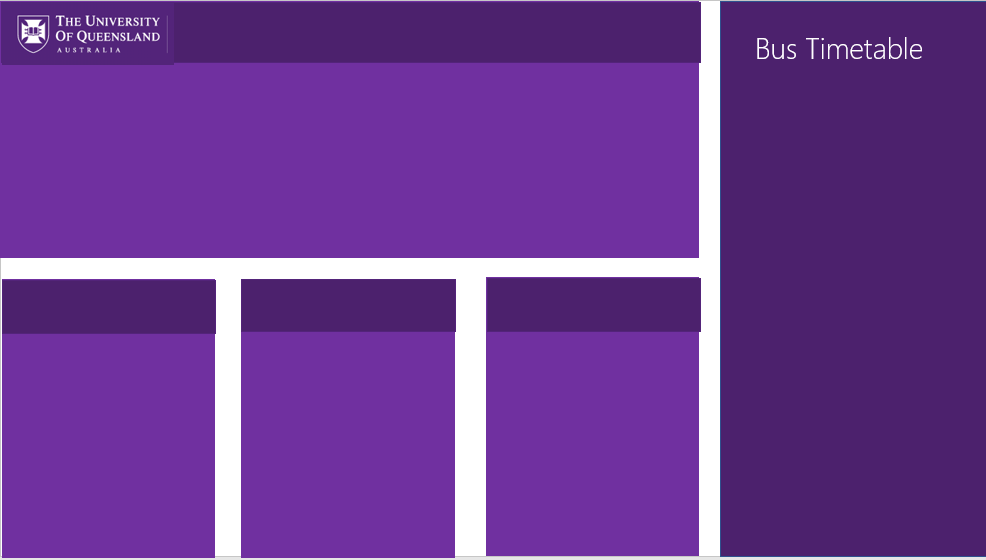
\includegraphics[width=0.8\textwidth]{Figures/UQlike.png}
			\caption{Display that has a ``UQ style" - 13/08/20}
			\label{UQlike}
		\end{figure}
		Here is the same colour scheme used with placeholder data and figures. \\
		
		\begin{figure}[h!]
			\centering
			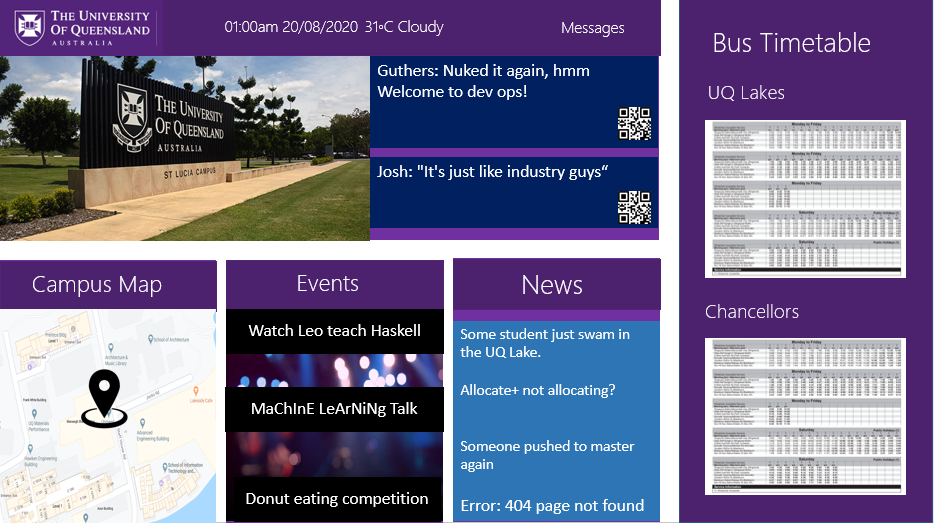
\includegraphics[width=0.8\textwidth]{Figures/UQlike2.png}
			\caption{Display that has a ``UQ style" (With placeholder data) - 13/08/20}
			\label{UQlike2}
		\end{figure}
		This colour scheme is fairly standard across UQ applications and services however, the front-end team decided to play around with other colour schemes that could blend display elements together more effectively whilst being easy on the eyes. Below are some of the different styles which were considered.
	
	\subsection{Back-End Progression}
		
	
\section{Issues During the Project}
	
	\subsection{How Issues Were Solved}

\section{Final Product \& Conclusion}
	
	\subsection{Figures}
	
	\subsection{Developer Thoughts}

\end{document}